\documentclass[a4wide, 11pt]{article}
\usepackage{a4, fullpage}
\setlength{\parskip}{0.3cm}
\setlength{\parindent}{0cm}
\usepackage{graphicx}

% This is the preamble section where you can include extra packages etc.

\begin{document}

\title{220 : Software Engineering Design - Othello}

\author{Leo Mak \and Miten Mistry\and Yufei Xie}

\date{\today}         % inserts today's date

\maketitle            % generates the title from the data above

\section{Introduction}
The main idea of this project was to recreate Othello and to properly design the implementation of the game. The idea of this report is to illustrate the various techniques, design patterns and concepts that have been implemented during the conceptualisation and creation of the game. There were several key areas that were considered during this process. These include the appropriate use of design patterns and their trades offs, the method in which code was developed, duplication of code and coupling.

\section{Using Java}
Java is an object-oriented language. The game board, players and pieces can all be viewed as objects that interact with each other, which naturally allows an object-oriented to efficiently model the game. Java runs on its own virtual machine meaning the game can be run on any operating system that has the Java Virtual Machine.

\section{UML diagram}
See next page.

\begin{figure}
\centering 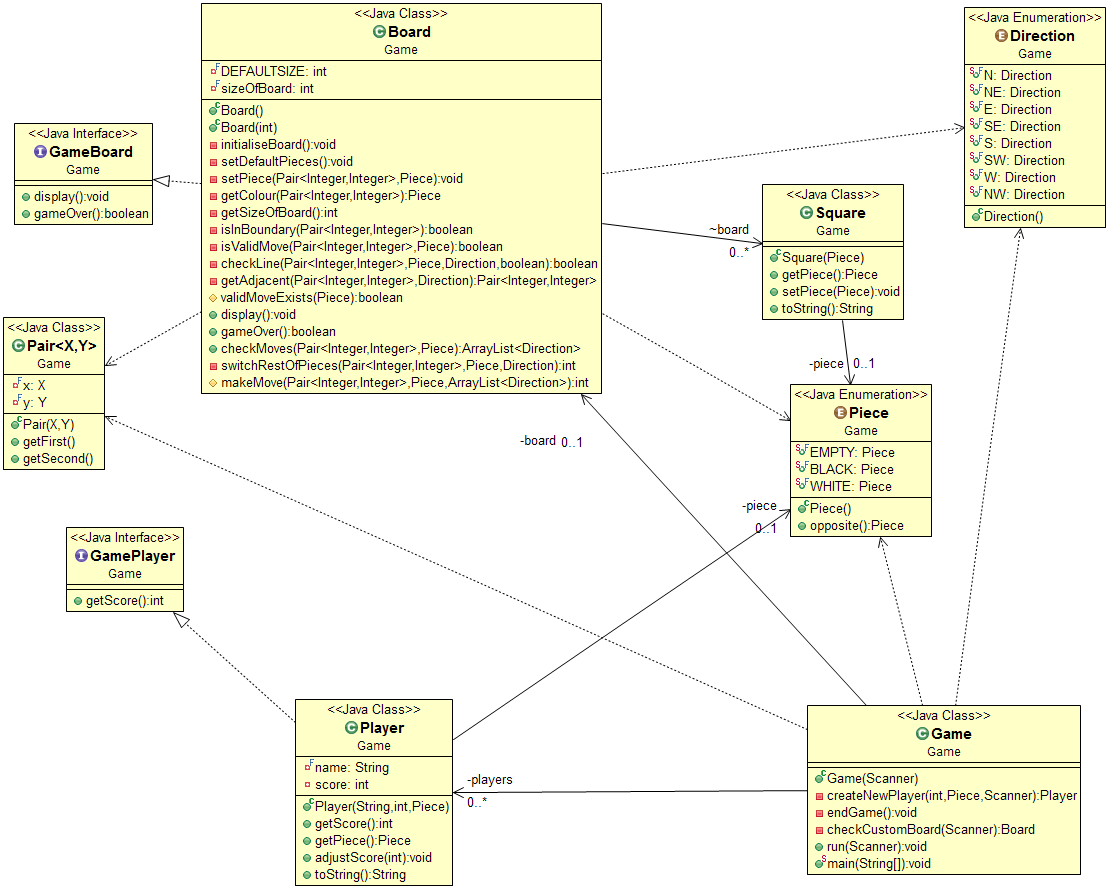
\includegraphics[width=180mm]{umlDiagram} 
\end{figure}


\subsection{Analysis on UML}
As the game can be interpreted as an object-oriented problem, it can be modeled by Unified Modeling Language, UML, see next page. The model contains two enumerated types: Piece and Direction; these represent the contents of a square on the board and the direction in which a move is valid from a particular point respectively.  Here enumerated types are an efficient design implementation as they allow the code to be understood easily and the enumerations can contain their own methods, i.e. how the enumerations can be represented if outputted. The diagram also contains interfaces, which can be used to extend the program to board games. A class containing generic types is also used, Pair, generic types allow a programmer to extend the same idea to sets of differing types hence removing duplicated code. The remaining classes represent a player, the Othello board and the game. The Game class handles input, output and the running of the game.

\section{Test Driven Development}
Upon creating the UML diagram, a basis of the design and functionality for the Othello game was established. Test cases were written based on the assumption that the completed code would behave as expected. Test driven development allowed test cases based on expectations of functionality to be written rather than focusing on how the code was written. However, while coding the program, certain features were changed that caused deviation from the UML, these changes may have occurred to allow a more efficient form of coding, causing some of the tests. Although there were limits to test driven development, the advantages outweighed the disadvantages as the tests were based on functionality, which allowed bugs to be discovered that may have been missed if tests were created based on how the methods were written. Once the tests had been passed, refactoring of the code was done, so that future programmers may easily interpret the code.

\section{Design Concepts}
\subsection{Abstaction and Refinement}
One of the first areas of design concepts that we considered was abstraction. The idea of generalising the content in order to retain relevant information was considered during the creation of the various classes. For example, if we take the class, Player, it is clearly displayed that the class is only relevant to players playing the game. Through the creation of an interface, a Computer player can be stemmed from the original player class with its methods overridden and other methods added. This class has reduced the necessary information for the player which as a result, allows the class to be used for a variety of different board games for example, Checkers which shows the idea of abstraction has been considered and used.  The idea of abstraction is further shown in the Board class whereby methods such as validation checks on going past the size of the board is considered whereas checking whether a move is valid can be overridden for other games. Control hierarchy was considered during the creation of the unified modelling language diagram to improve the use of object orientation.

Refinement through the process of elaboration is also demonstrated throughout the program where instructions are decomposed into more detailed instructions. An excellent example of this would be in the initialisation of the Board where the board is created and subsequently, the default starting positions are added onto the board. During the start of the game, the program will call for the creation of the board which then leads to the generation of an empty board which then allows the default pieces to be added. The idea of refinement is clearly exhibited, as instructions are decomposed into more detailed instruction methods which are called by the previous method. This is an ideal augmentation to abstraction since the initial eight by eight can be generated but through the use of abstraction, the method for the default layout can be overridden for a different game, such as Chess. As a result, the difficulty of the task has been reduced thanks to the discipline of software architecture during the use of abstraction and refinement.

\subsection{Modularity and Structural Partitioning}
The idea of modularity has also been shown whereby the program has been split into multiple classes to maximise object orientation which allows us to effectively manage our program. Furthermore, through the use of packages, test cases are separated from the main program, to ensure test driven development is fully utilised. Both horizontal and vertical partitioning have both been used during the development of Othello. Horizontal partitioning has been used during the processing of input moves where the input is taken and passed through the Board class where the move is validated, and the Game class which carries out the move. The advantage of this is that testing, maintaining and in the future, extending the code is easy to do and there is also far less side effects in change or error propagation. The biggest issue with using horizontal partitioning is that since data is passed around throughout the program, it makes the program slightly more complex but this problem is far overshadowed by the benefits. The program has been handled in a top down approach which makes it easier to handle and maintain any changes that will or have been made.

\subsection{Encapsulation and Data Structures}
An effort has also been made to conceal any methods which do not need to be visible from anything that does not need to call it. Though the use of encapsulation, the integrity of the program is also maintained and the complexity is also reduced since there are few interdependencies between modules. For example, in the Board class, certain methods are defined to be private as they are only called within the class, so visibility is minimised. Data structures are also used to simplify the implementation as well as make the program easy to understand. An arraylist has been implemented to store the directions in which pieces can be captured to make it easier to handle during processing. Furthermore, a data structure named pairwas created, which will allow the coordinates of each move to be stored and processed. This makes using the board much easier since rather than passing two separate parameters for the coordinates, they are placed in one data structure which makes the system much more robust. An enumeration is also used to store the status of each square to remove any possible amibuiguities from the program.

\section{Design Patterns}
Listed below are a few of the design patterns that have been incorporated into the program:
\begin{itemize}

    \item Abstract Factory - The use of interfaces to create dependent classes. This was used when creating the Board and Player classes to allow the program to be extended to other games.

    \item Builder - The process of separation the construction of an object to increase functionality. This was used in the Board class to allow custom and default sized boards to be handled.

    \item Module Pattern - Grouping related elements into one. This is shown by the use of separate packages for the tests and the game files.
    
\end{itemize}
\section{Design Considerations}

\begin{itemize}

    \item Compatibility and Maintainability – As a result of using Java, the program can be executed on any computer architecture; the program is cross platform compatible. In terms of maintainability, comments have been added to further clarify any ambiguous or confusing code. Accurate identifier names have also been used so the program is easily understandable. Furthermore, due to modularity, we have independent classes which is easier to maintain.

   \item Extensibility, Reusability and Modularity – New features, capabilities and modifications can be easily added into the program since we have used modularity to separate classes. This means that they can be independently tested in isolation before being integrated into the program. Furthermore, through the use of interfaces, methods can be overridden and new features can be added without changing any existing code. 

   \item Robustness and Usability – The program that has been created has been designed to be robust and easily usable. If wrong input is entered when deciding on the size of the board, the player name or the player's move, accurate and helpful error statements are provided to the user. The user is subsequently asked to enter a valid input. Through the use of structural partitioning, the program demonstrates further that it is robust. The program is easy to use since it has clear and helpful commands for the user and the board is accurately depicted. 
 
\end{itemize}

\section{Consequences of our design choices}
In terms of coupling and cohesion, the program currently has data coupling, where modules share data only through parameters and there are no other ways in which data is shared. The advantage of this is that if one module changes, it shouldn't have much of an effect on another module since data is only passed through the parameters and unless they are changed, it should not affect another module. Another advantage of low coupling is that modules can be reused as a result. In terms of cohesion, the program currently has high cohesion since methods are strongly related to another and they carry out similar processes to each other. For example, in the player class, every method and variable is directly related to a player and there are no unnecessary variables. The consequence of this is that both code reuse and readability are increased in effectiveness and classes are robust and reliable. As demonstrated in both the screenshot and the test driven development, the program is functionally correct and is robust, so incorrect inputs are rejected. The program is quite flexible since we have the implementation of interfaces and by splitting up the methods into many separate methods, it can easily be modified through the overwriting different classes.


\section{Screenshot demonstrating Othello}
Shown below are two screenshots of Othello working, one a default game and another, a custom game.

\begin{figure}
\centering \includegraphics[width=150mm,height=200mm]{reversi} 
\end{figure}

\end{document}


